% GNUPLOT: LaTeX picture with Postscript
\begingroup
  \makeatletter
  \providecommand\color[2][]{%
    \GenericError{(gnuplot) \space\space\space\@spaces}{%
      Package color not loaded in conjunction with
      terminal option `colourtext'%
    }{See the gnuplot documentation for explanation.%
    }{Either use 'blacktext' in gnuplot or load the package
      color.sty in LaTeX.}%
    \renewcommand\color[2][]{}%
  }%
  \providecommand\includegraphics[2][]{%
    \GenericError{(gnuplot) \space\space\space\@spaces}{%
      Package graphicx or graphics not loaded%
    }{See the gnuplot documentation for explanation.%
    }{The gnuplot epslatex terminal needs graphicx.sty or graphics.sty.}%
    \renewcommand\includegraphics[2][]{}%
  }%
  \providecommand\rotatebox[2]{#2}%
  \@ifundefined{ifGPcolor}{%
    \newif\ifGPcolor
    \GPcolortrue
  }{}%
  \@ifundefined{ifGPblacktext}{%
    \newif\ifGPblacktext
    \GPblacktexttrue
  }{}%
  % define a \g@addto@macro without @ in the name:
  \let\gplgaddtomacro\g@addto@macro
  % define empty templates for all commands taking text:
  \gdef\gplbacktext{}%
  \gdef\gplfronttext{}%
  \makeatother
  \ifGPblacktext
    % no textcolor at all
    \def\colorrgb#1{}%
    \def\colorgray#1{}%
  \else
    % gray or color?
    \ifGPcolor
      \def\colorrgb#1{\color[rgb]{#1}}%
      \def\colorgray#1{\color[gray]{#1}}%
      \expandafter\def\csname LTw\endcsname{\color{white}}%
      \expandafter\def\csname LTb\endcsname{\color{black}}%
      \expandafter\def\csname LTa\endcsname{\color{black}}%
      \expandafter\def\csname LT0\endcsname{\color[rgb]{1,0,0}}%
      \expandafter\def\csname LT1\endcsname{\color[rgb]{0,1,0}}%
      \expandafter\def\csname LT2\endcsname{\color[rgb]{0,0,1}}%
      \expandafter\def\csname LT3\endcsname{\color[rgb]{1,0,1}}%
      \expandafter\def\csname LT4\endcsname{\color[rgb]{0,1,1}}%
      \expandafter\def\csname LT5\endcsname{\color[rgb]{1,1,0}}%
      \expandafter\def\csname LT6\endcsname{\color[rgb]{0,0,0}}%
      \expandafter\def\csname LT7\endcsname{\color[rgb]{1,0.3,0}}%
      \expandafter\def\csname LT8\endcsname{\color[rgb]{0.5,0.5,0.5}}%
    \else
      % gray
      \def\colorrgb#1{\color{black}}%
      \def\colorgray#1{\color[gray]{#1}}%
      \expandafter\def\csname LTw\endcsname{\color{white}}%
      \expandafter\def\csname LTb\endcsname{\color{black}}%
      \expandafter\def\csname LTa\endcsname{\color{black}}%
      \expandafter\def\csname LT0\endcsname{\color{black}}%
      \expandafter\def\csname LT1\endcsname{\color{black}}%
      \expandafter\def\csname LT2\endcsname{\color{black}}%
      \expandafter\def\csname LT3\endcsname{\color{black}}%
      \expandafter\def\csname LT4\endcsname{\color{black}}%
      \expandafter\def\csname LT5\endcsname{\color{black}}%
      \expandafter\def\csname LT6\endcsname{\color{black}}%
      \expandafter\def\csname LT7\endcsname{\color{black}}%
      \expandafter\def\csname LT8\endcsname{\color{black}}%
    \fi
  \fi
  \setlength{\unitlength}{0.0500bp}%
  \begin{picture}(5040.00,2880.00)%
    \gplgaddtomacro\gplbacktext{%
      \colorrgb{0.61,0.61,0.61}%
      \put(438,1047){\makebox(0,0)[r]{\strut{}\footnotesize{0}}}%
      \colorrgb{0.61,0.61,0.61}%
      \put(438,1278){\makebox(0,0)[r]{\strut{}\footnotesize{20}}}%
      \colorrgb{0.61,0.61,0.61}%
      \put(438,1509){\makebox(0,0)[r]{\strut{}\footnotesize{40}}}%
      \colorrgb{0.61,0.61,0.61}%
      \put(438,1740){\makebox(0,0)[r]{\strut{}\footnotesize{60}}}%
      \colorrgb{0.61,0.61,0.61}%
      \put(438,1971){\makebox(0,0)[r]{\strut{}\footnotesize{80}}}%
      \colorrgb{0.61,0.61,0.61}%
      \put(438,2202){\makebox(0,0)[r]{\strut{}\footnotesize{100}}}%
      \colorrgb{0.61,0.61,0.61}%
      \put(438,2433){\makebox(0,0)[r]{\strut{}\footnotesize{120}}}%
      \colorrgb{0.61,0.61,0.61}%
      \put(976,888){\rotatebox{45}{\makebox(0,0)[r]{\strut{}\footnotesize{bgm}}}}%
      \colorrgb{0.61,0.61,0.61}%
      \put(1416,888){\rotatebox{45}{\makebox(0,0)[r]{\strut{}\footnotesize{stereovision0}}}}%
      \colorrgb{0.61,0.61,0.61}%
      \put(1855,888){\rotatebox{45}{\makebox(0,0)[r]{\strut{}\footnotesize{stereovision1}}}}%
      \colorrgb{0.61,0.61,0.61}%
      \put(2295,888){\rotatebox{45}{\makebox(0,0)[r]{\strut{}\footnotesize{LU8PEEng}}}}%
      \colorrgb{0.61,0.61,0.61}%
      \put(2734,888){\rotatebox{45}{\makebox(0,0)[r]{\strut{}\footnotesize{mkDelayWorker32B}}}}%
      \colorrgb{0.61,0.61,0.61}%
      \put(3173,888){\rotatebox{45}{\makebox(0,0)[r]{\strut{}\footnotesize{stereovision2}}}}%
      \colorrgb{0.61,0.61,0.61}%
      \put(3613,888){\rotatebox{45}{\makebox(0,0)[r]{\strut{}\footnotesize{mcml}}}}%
      \colorrgb{0.61,0.61,0.61}%
      \put(4052,888){\rotatebox{45}{\makebox(0,0)[r]{\strut{}\footnotesize{LU32PEEng}}}}%
      \colorrgb{0.61,0.61,0.61}%
      \put(4492,888){\rotatebox{45}{\makebox(0,0)[r]{\strut{}\footnotesize{geomean}}}}%
      \csname LTb\endcsname%
      \put(48,1740){\rotatebox{-270}{\makebox(0,0){\strut{}\footnotesize{\textbf{Critical Path Delay (ns)}}}}}%
      \put(2734,42){\makebox(0,0){\strut{}\footnotesize{\textbf{Circuit}}}}%
    }%
    \gplgaddtomacro\gplfronttext{%
      \csname LTb\endcsname%
      \put(816,2739){\makebox(0,0)[l]{\strut{}\footnotesize{No Partitioning (Base Flow)}}}%
      \csname LTb\endcsname%
      \put(816,2582){\makebox(0,0)[l]{\strut{}\footnotesize{Packing Constraints Only}}}%
      \csname LTb\endcsname%
      \put(3039,2739){\makebox(0,0)[l]{\strut{}\footnotesize{Placement Constraints Only}}}%
      \csname LTb\endcsname%
      \put(3039,2582){\makebox(0,0)[l]{\strut{}\footnotesize{Packing and Placement Constraints}}}%
    }%
    \gplbacktext
    \put(0,0){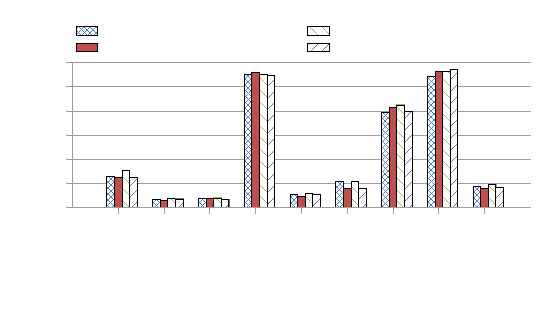
\includegraphics{vpr_flows_crit_path}}%
    \gplfronttext
  \end{picture}%
\endgroup
